\begin{table}[H]
    \caption{Percentage contribution of group members}
    \begin{center}
        \begin{tabular}{||c|c|c||}
            \hline
            \multicolumn{3}{||c||}{\textbf{Group 21}}                            \\
            \hline
            \textbf{Name}   & \textbf{Contribution \%} & \textbf{Student number} \\
            \hline
            \hline
            Haochen Yang    & 20                       & 19061935                \\
            Muhammad Naveed & 20                       & 19006675                \\
            Yikai Zhang     & 20                       & 19009845                \\
            Ryan El Khoury  & 20                       & 19084828                \\
            Hasha Dar       & 20                       & 19090799                \\
            \hline
        \end{tabular}
    \end{center}
\end{table}
\section{Introduction to Lift and Drag}
\subsection{Description of lift and drag}
A fluid, for example air in our case, that flows around an object will act a force on it. In our case, this object is the airfoil. Lift is the effect of the force applied by the fluid in the perpendicular direction to the flow direction. The lift force can be calculated with known pressure distribution.
\begin{align}
    L = \oint \left(p n k \right)\dif S
\end{align}
Where $p$ is the pressure on the surface of the airfoil, $n$ is the normal unit vector pointing into the wing, $k$ is the vertical unit vector, normal to the airfoil direction. Or it can be calculated by using lift coefficient:
\begin{align}
    L = \frac{1}{2} \rho V^2 A C_l
\end{align}
Where $\rho$ is the density of the fluid (air), $V$ is the velocity of the flow and $A$ is the wing area. Drag is also called fluid resistance because it acts like a resistance force. Drag acts opposite to the motion of any object with respect to the fluid that flows around it. Drag can also be calculated as:
\begin{align}
    D = \frac{1}{2} \rho V^2 A C_d
\end{align}
Where $C_d$ is the drag coefficient.
\begin{figure}[H]
    \centering
    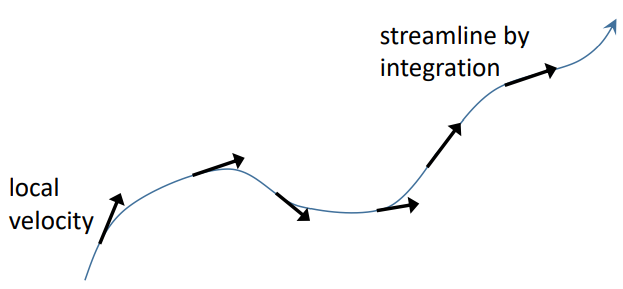
\includegraphics[width = 0.5 \textwidth]{./img/diagram1.png}
    \caption{}
\end{figure}
\subsection{Description of the difference between form and friction drags, and how their contribution differ in streamlined and bluff bodies}
\begin{figure}[H]
    \centering
    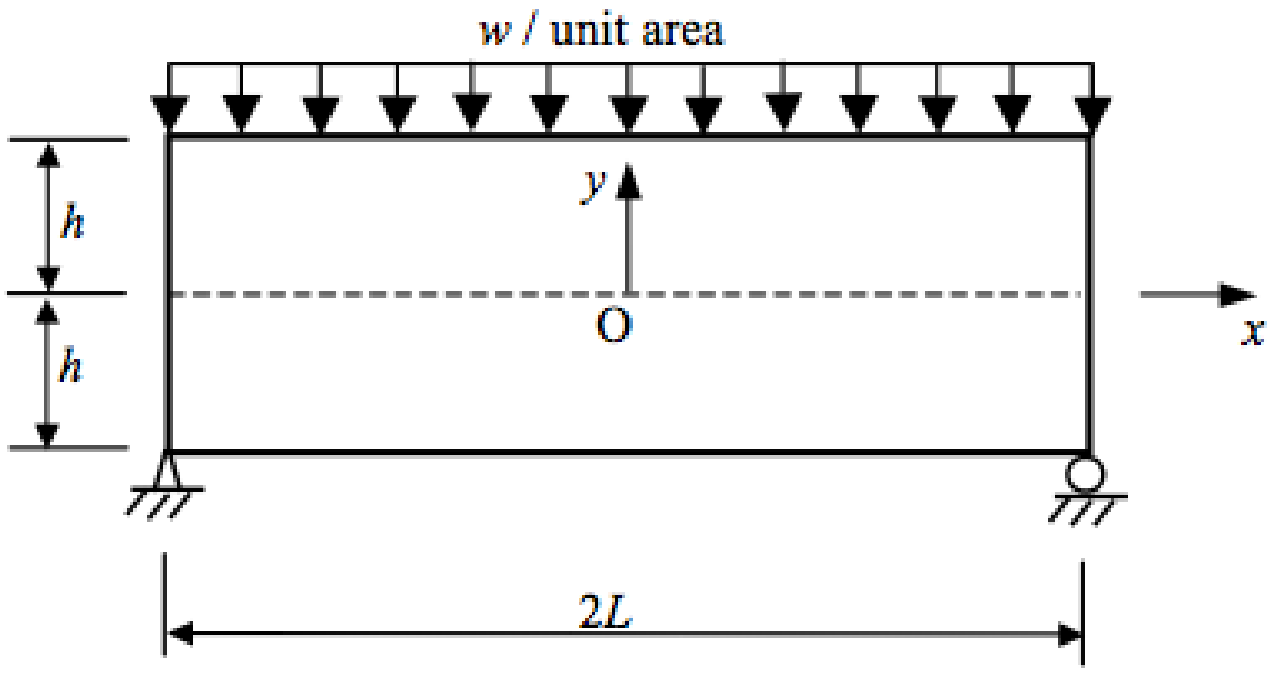
\includegraphics[width = 0.5 \textwidth]{./img/diagram2.png}
    \caption{}
\end{figure}
Force generated by pressure can be written as:
\begin{align}
    F = p \dif S
\end{align}
Where $p$ is the pressure on the surface area $\dif S$. Form drag is the normal component of the force normal to the surface. Hence, the form drag can be calculated by integrating the force component in the stream direction iver the whole surface area.
\begin{align}
    D_f = \int_S \left(p\right)\dif S
\end{align}
The skin friction is the tangential component of the force normal to the surface. Hence, skin friction can be calculated by integrating the shear force, $\tau_w \dif S$, over the whole area.
\begin{align}
    F_s = \int_S \left(\tau_w\right)\dif S
\end{align}
\subsection{Determination of the lift coefficient of a finite wing utilising the coefficient of an infinite one. Explanation on why this is necessary and what measures can be taken to improve the efficiency of a wing}
The lift coefficient of the finite wing can be calculated with given lift coefficient of a finite wing by using lifting-line theory.
\begin{figure}[H]
    \centering
    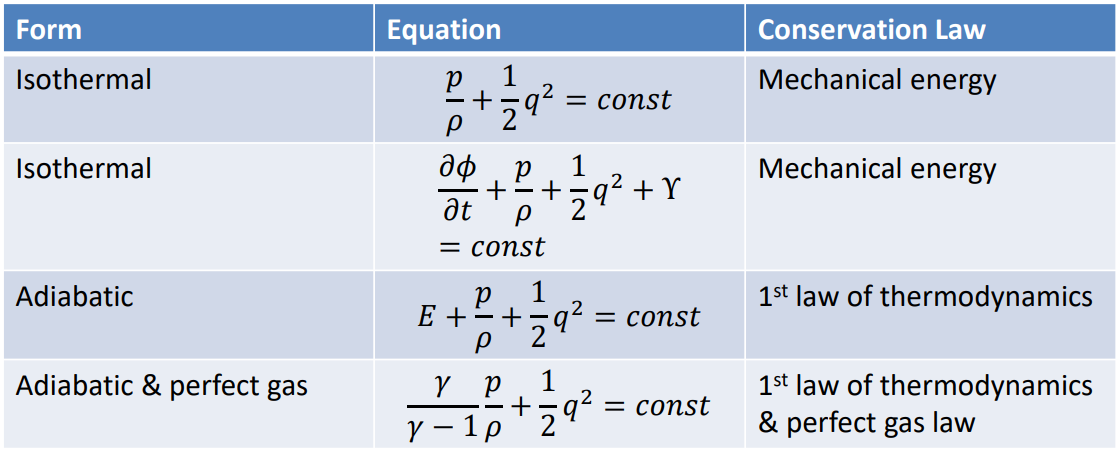
\includegraphics[width = 0.35 \textwidth]{./img/diagram3.png}
    \caption{For a given wing with wing span $b$ and chord length $c$}
\end{figure}
\begin{figure}[H]
    \centering
    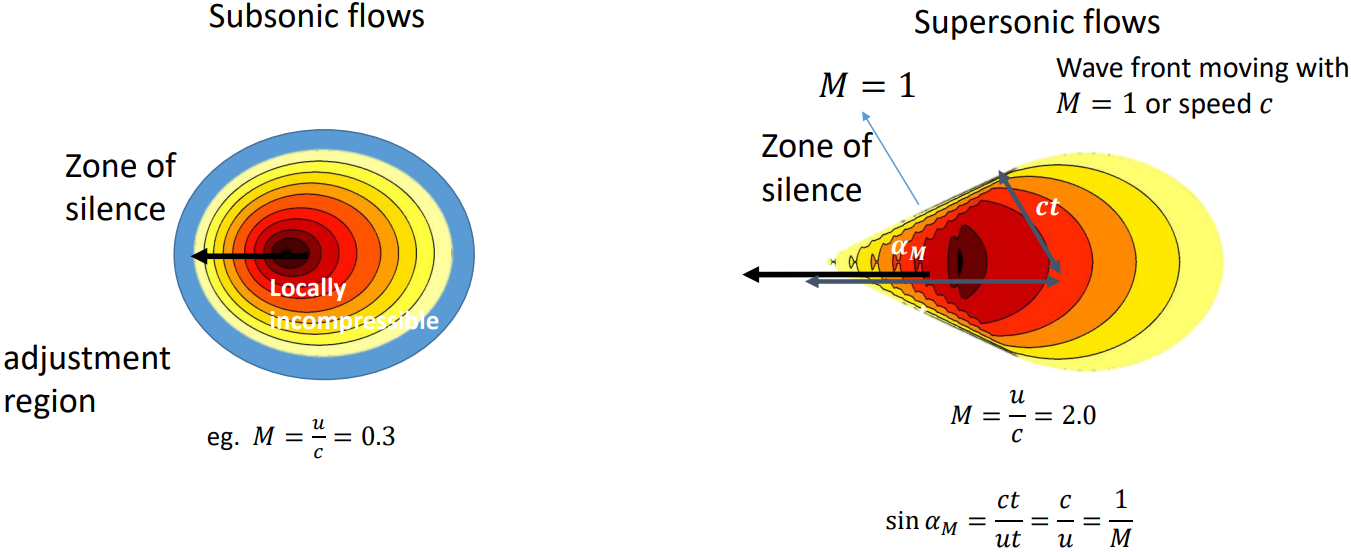
\includegraphics[width = 0.5 \textwidth]{./img/diagram4.png}
    \caption{}
    \label{GeometricAngleOfAttack}
\end{figure}
As shown in the graph, the geometric angle of attack is $\alpha$ and $\alpha_e$ is the effective geometry of angle of attack. $\alpha_i$ is the induced angle of attack. $V_{\infty}$ is the free stream flow velocity, $W$ is the downwash caused by the flow and $\alpha_e = \alpha - \alpha_i$.

Also, by applying the \textit{Biot-Savart} Law,  for a given vortex filament with strength $\Gamma$, the velocity of a certain point $P$ which is created by this vortex
\begin{figure}[H]
    \centering
    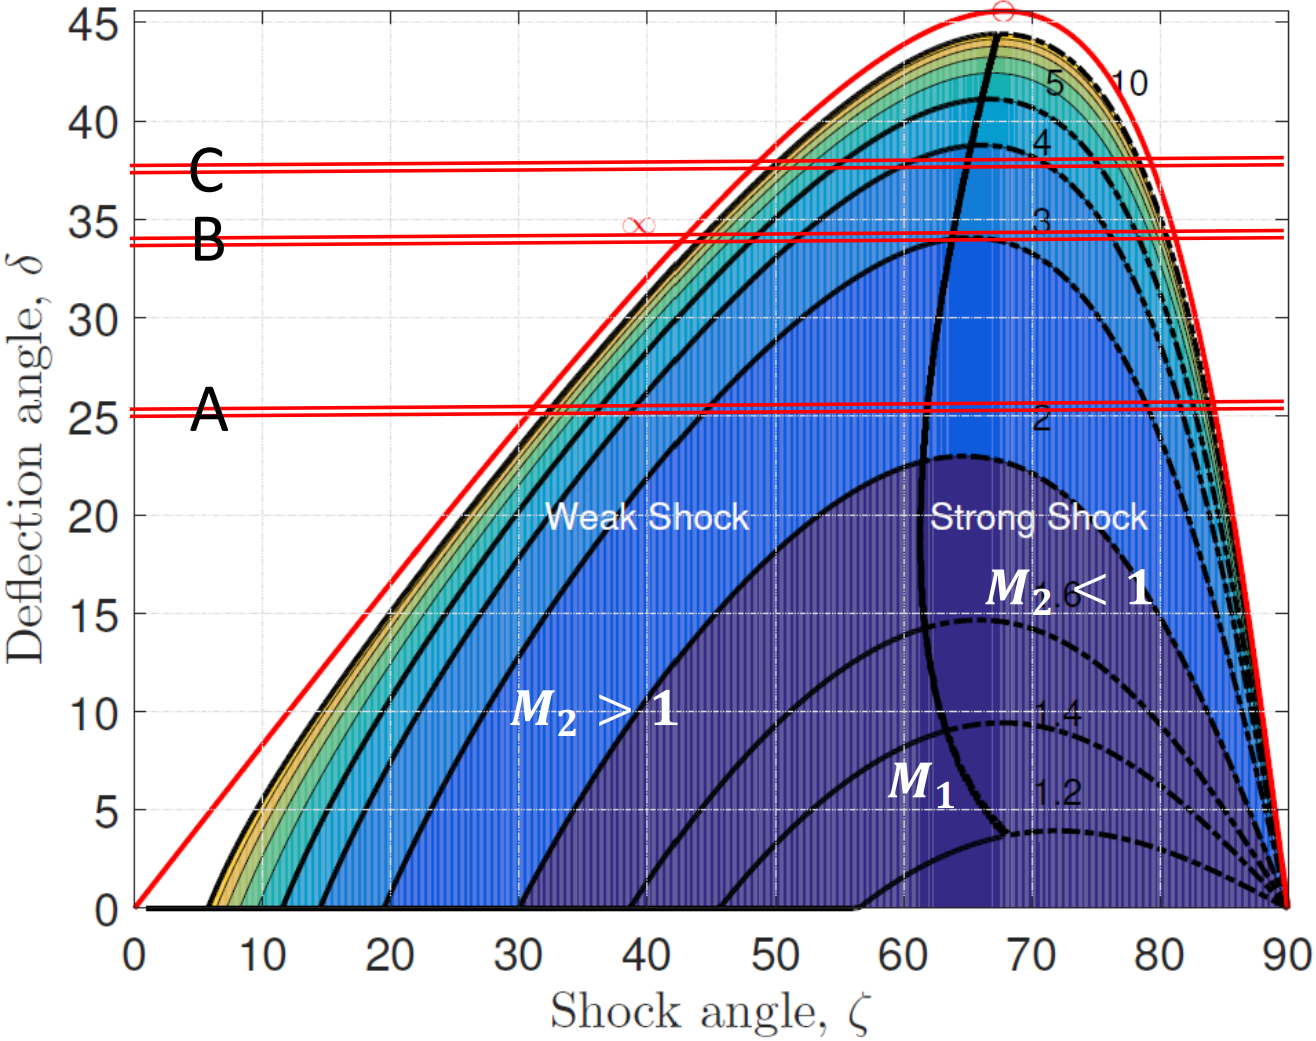
\includegraphics[width=0.2\textwidth]{./img/diagram5.png}
    \caption{}
\end{figure}
\begin{align}
    \left| \vec{V} \right| & = \frac{\Gamma}{4\pi} \int_{-\infty}^{\infty} \frac{\left| \dif \vec{l} \cdot \vec{r} \right| }{ \left| r \right|^3} \\
    l                      & = r\cos{\theta}                                                                                                      \\
    h                      & = r\sin{\theta}                                                                                                      \\
    \dif l                 & = -\frac{h}{\sin{\theta}}                                                                                            \\
    \left| \vec{V} \right| & = \frac{\Gamma}{4\pi} \int_{\pi}^0 \left(\frac{-\sin{\theta}}{h}\right) \dif \theta                                  \\
\end{align}
So the downwash at a certain point on the wing will be:
\begin{align}
    W = \frac{\Gamma}{4\pi h} \int_{\frac{\pi}{2}}^0\left(-\sin{\theta}\right)\dif \theta = \frac{\Gamma}{4\pi h}
\end{align}
The lift per unit span:
\begin{align}
    L_v      & = \rho V_{\infty} \Gamma = \frac{1}{2}\rho V_{\infty}^2 c C_l = \frac{1}{2} \rho V_{\infty}^2 c \cdot 2\pi \alpha_e \\
    \Gamma   & = cV_{\infty}\pi \left(\alpha - \alpha_i\right)                                                                     \\
    \alpha_i & = \frac{-w\left(y\right)}{V_{\infty}}
\end{align}
However when we are considering the downwash at the wing tips where $h=0$. The angle of attack is approach infinity, but that's impossible. So, we introduce the lifting-line theory. We suggest that $\gamma$ is a function of $y$. But according to \textit{Helmholtz's} first theorem, the strength of a vortex filament is a constant along its length. So, in order to let $\Gamma$ to change $y$ along y, we create an infinitely large number of trailing vortexes which all have slightly different strengths.
\begin{align}
    \dif \Gamma                  & = \frac{\dif \Gamma}{\dif y} \dif y                                                                                                                                      \\
    \therefore W\left(y_0\right) & = \int_{\frac{-b}{2}}^{\frac{b}{2}} \left(\frac{\frac{\dif \Gamma}{\dif y}}{4\pi \left(y-y_0\right)}\right) \dif y                                                       \\
    C_l                          & = \frac{2\Gamma\left(y_0\right)}{V_{\infty}c\left(y_0\right)} = 2\pi \alpha_e = 2\pi\left(\alpha\left(y_0\right) - \alpha_i \left(y_0\right)\right)                      \\
    \alpha_i \left( y_0 \right)  & = -\frac{w\left( y_0 \right)}{V_{\infty}} = -\frac{1}{4\pi V_{\infty}} \int_{\frac{-b}{2}}^{\frac{b}{2}} \left( \frac{\frac{\dif \Gamma}{\dif y}\dif y}{y - y_0} \right) \\
    \Gamma \left(y\right)        & = \Gamma \left(y_0\right) \sqrt{1 - \left(\frac{2y}{b}\right)^2}                                                                                                         \\
    \frac{\dif \Gamma}{\dif y}   & = -\frac{4\Gamma_0 y}{b^2} \left(\sqrt{1-\left(\frac{2y}{b}\right)^2}\right)^{-1}                                                                                        \\
    \therefore w\left(y_0\right) & = -\frac{\Gamma_0}{2b}
\end{align}
Where - point is the mid point of the wingspan. The lift of the finite wing is:
\begin{align}
    L   & = \int_{\frac{-b}{2}}^{\frac{b}{2}} \left(L\left(y\right)\right)\dif y = \rho V_{\infty} \Gamma_0 \int_{\frac{-b}{2}}^{\frac{b}{2}} \sqrt{1-\left(\frac{2y}{b}\right)^2} \dif y = \frac{1}{4}\rho \Gamma_0 b\pi \\
    C_L & = \frac{L}{\frac{1}{2}\rho V_{\infty}^2 S} = \frac{\Gamma_0 b \pi}{2V_{\infty S}}
\end{align}
It is usually hard to calculated the lift force of the whole wing in the three dimensional world. So, it is much more easier just to consider slicing the wing into cross-section. But we can’t just add up all the independently calculated forces of each cross-section because this approximation is incorrect. In practice, each cross-sectionof the wing will influence its neighbouring one. The lifting-line theory correct part of the errors by introducing the interactions between the wing slices.

To maximize the efficiency of the wing, we must maximize the lift force exerted on the wing surface. To achieve that, we must minimize the downwash at the wing tips. One of the way to do so is to change the wing tip by adding a winglet.
\section{Part 1 - Experimental Data Processing}
\subsection{Description of the experimental apparatus, the experimental procedure and sources of error. Explanation on why negative pressures are measured}
The goal of this experiment is to measure the pressure around the airfoil. Pressure tappings are located on the upper and lower surfaces of the airfoil. These tappings are connected to a manometer using tubes. The multi-tube manometer is filled with coloured water, and half of it is connected to the pressure tappings of the airfoil and measures the pressure different point on the its surfaces, and the other half is left unconnected, and measures the atmospheric pressure of the room. The airfoil is placed in an air tunnel, and can be rotated with the help of a remote controlled stepper motor. Next, the wind tunnel velocity (free stream total) can be calculated using $P_{tot}$ which is measured with a pitot tube inside the wind tunnel, $P_{inf}$ which is measured by a pressure tapping on the wall of the wind tunnel, and the air density which is given. The sources of errors can come from an air leakage, an imprecise angle of attack, non-negligible drag and lift forces on the support of the wing (test rig). All the measured pressures are inferior than $P_{atm}$ which is measured by the tube 21, so they are all negative with respect to the measured atmospheric pressure - this creates a vacuum at the top and bottom surfaces of the airfoil. However, when the angle of attack is between 0 and 18 degrees, the pressure at the top is lower than the pressure at the bottom, lifting the airfoil upwards.
\subsection{Determination of the free stream velocity, $U_{\infty}$, and the Reynolds number, $Re$}
The free stream can be calculated as such:
\begin{align}
    U_{\infty} = \sqrt{\frac{2}{\rho}\left(P_{tot} - P_{inf}\right)} = \sqrt{\frac{2}{1.23}\left( \left| 42-71 \right| \right) \cdot 9.80638} = \SI{20.50}{\meter\per\second}
\end{align}
The Reynolds number can be calculated as such:
\begin{align}
    Re = \frac{\rho v l}{\mu} = \frac{1.23 \cdot 6.87 \cdot 0.15}{1.938\cdot 10^{-5}} = 63919
\end{align}
\subsection{Determination of pressure coefficient, $c_p$, for each angle of attack of the upper and lower surface with tabulated data}
\begin{figure}[H]
    \centering
    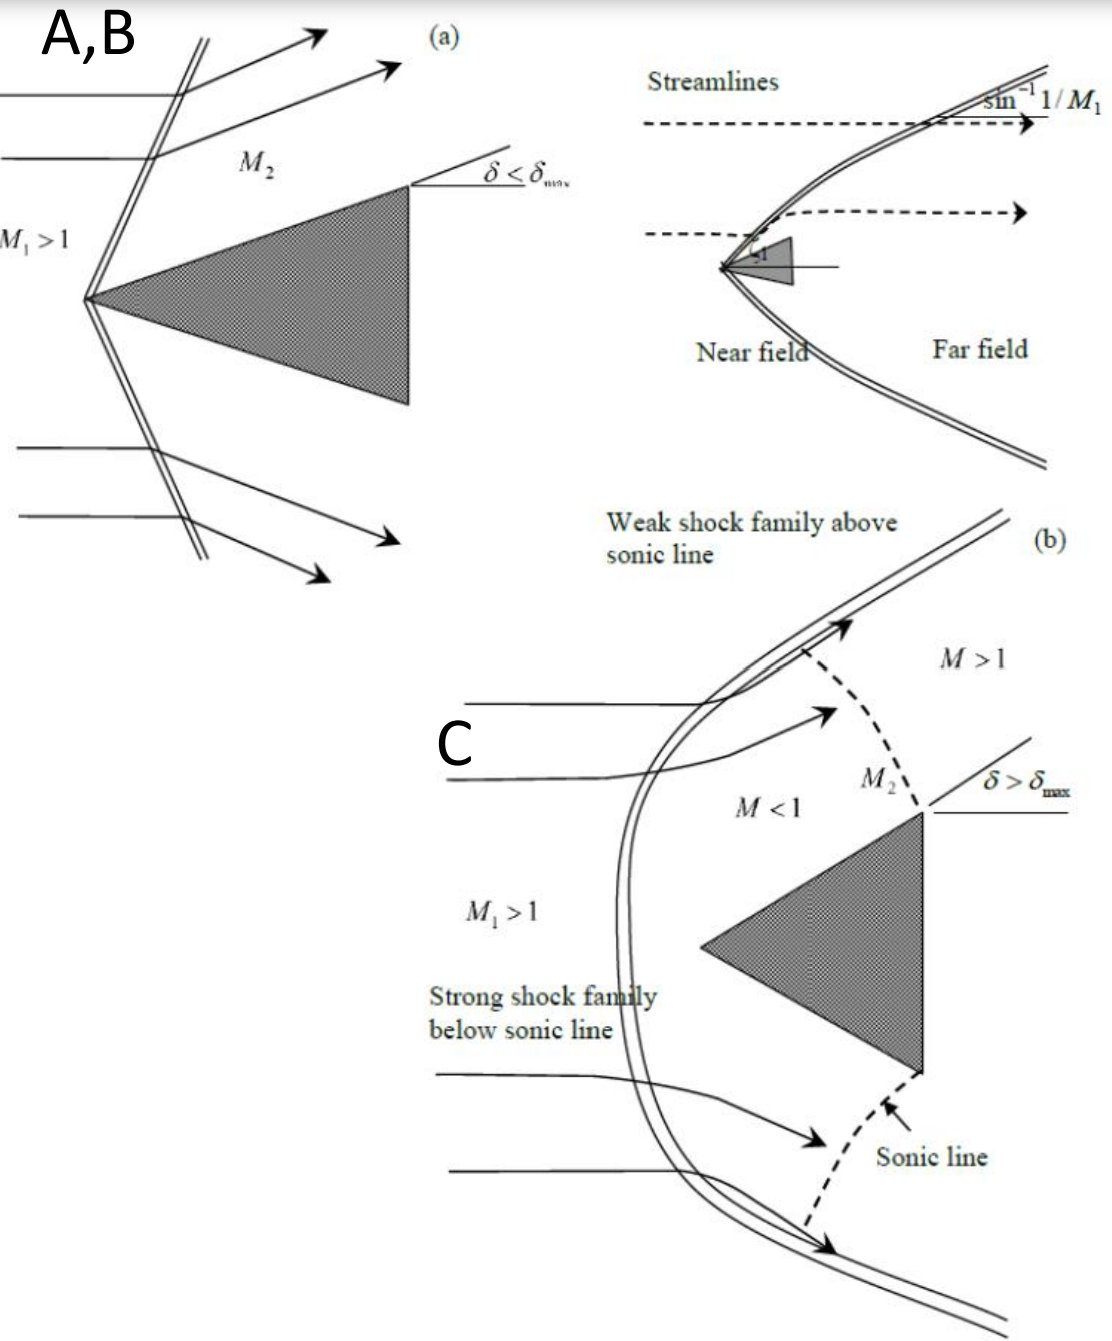
\includegraphics[width=0.9\textwidth]{./img/diagram6.png}
    \caption{Measured pressure (in mmH20) of the tappings at each angle.}
\end{figure}
\begin{figure}[H]
    \centering
    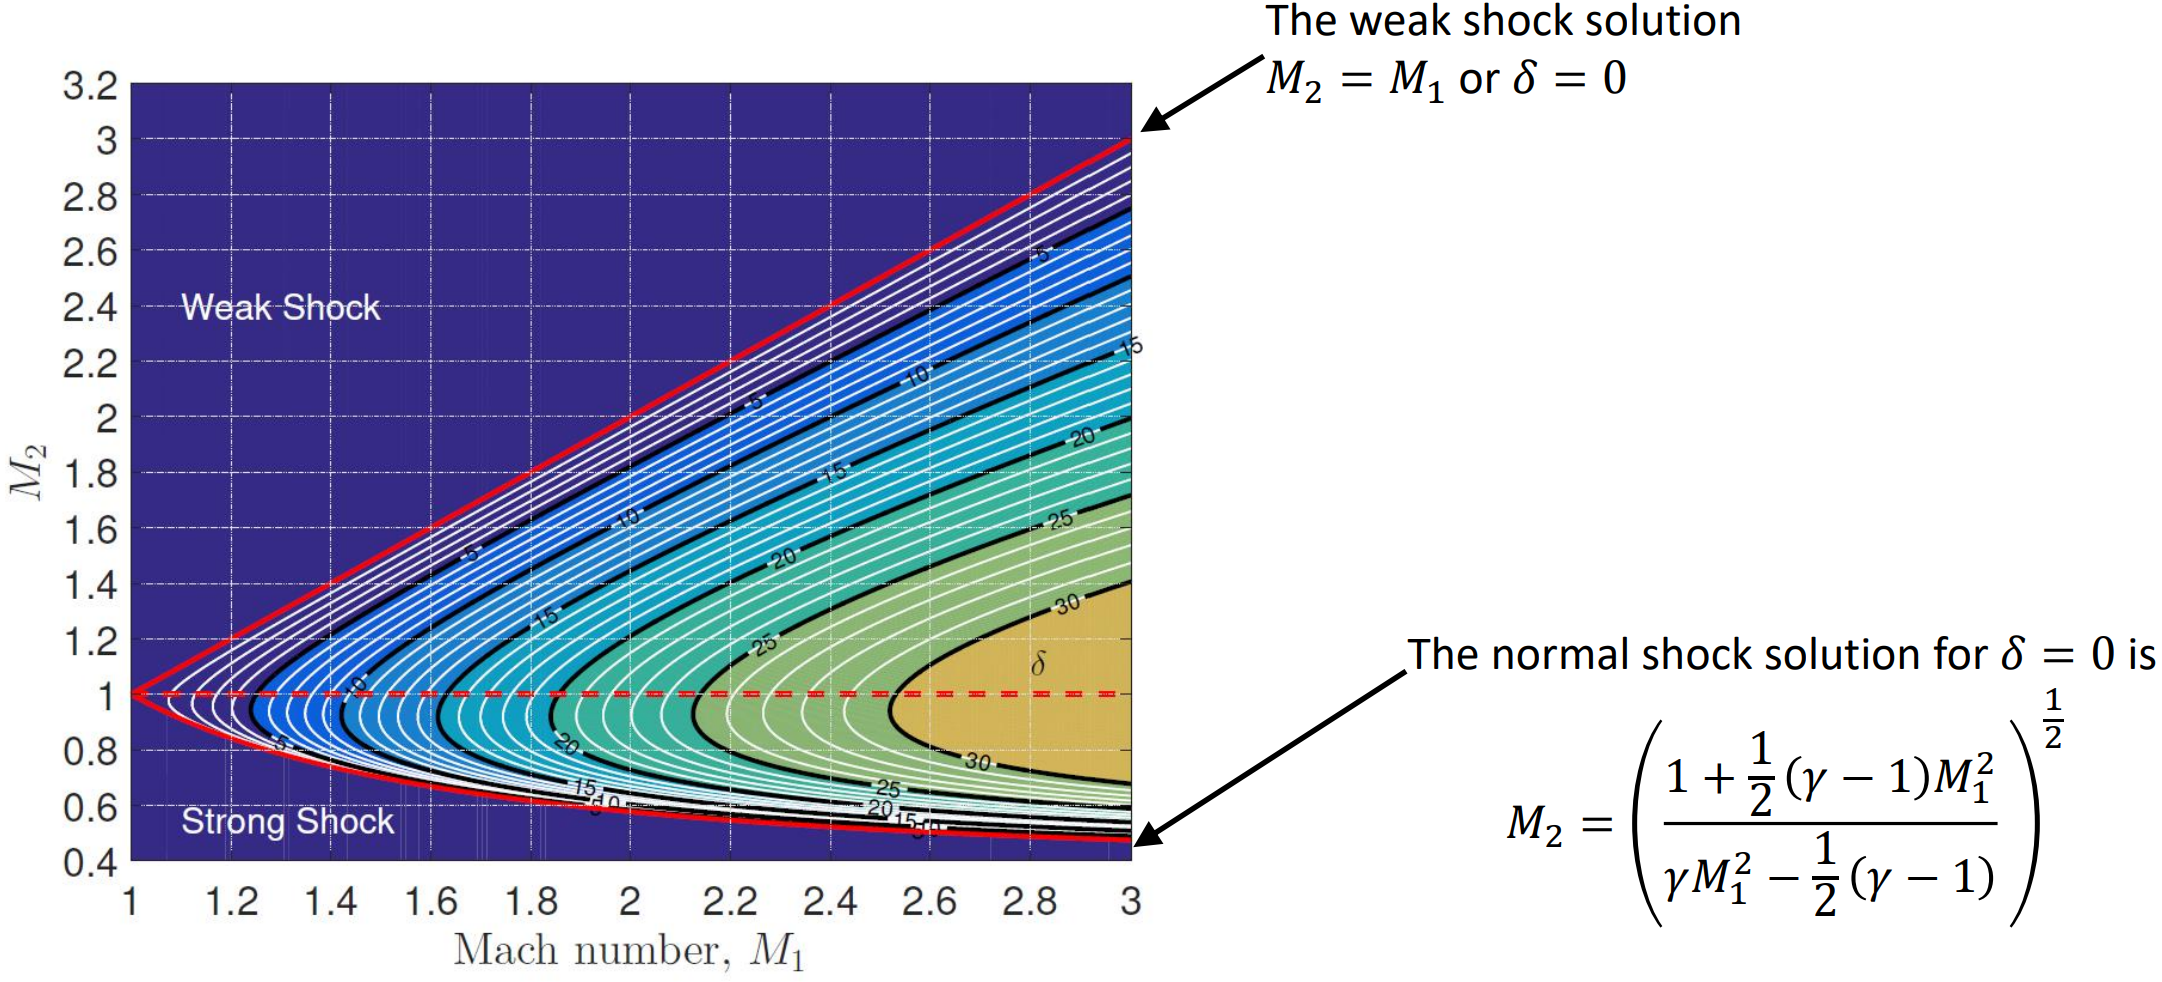
\includegraphics[width=0.9\textwidth]{./img/diagram7.png}
    \caption{Water height differences.}
\end{figure}
\begin{figure}[H]
    \centering
    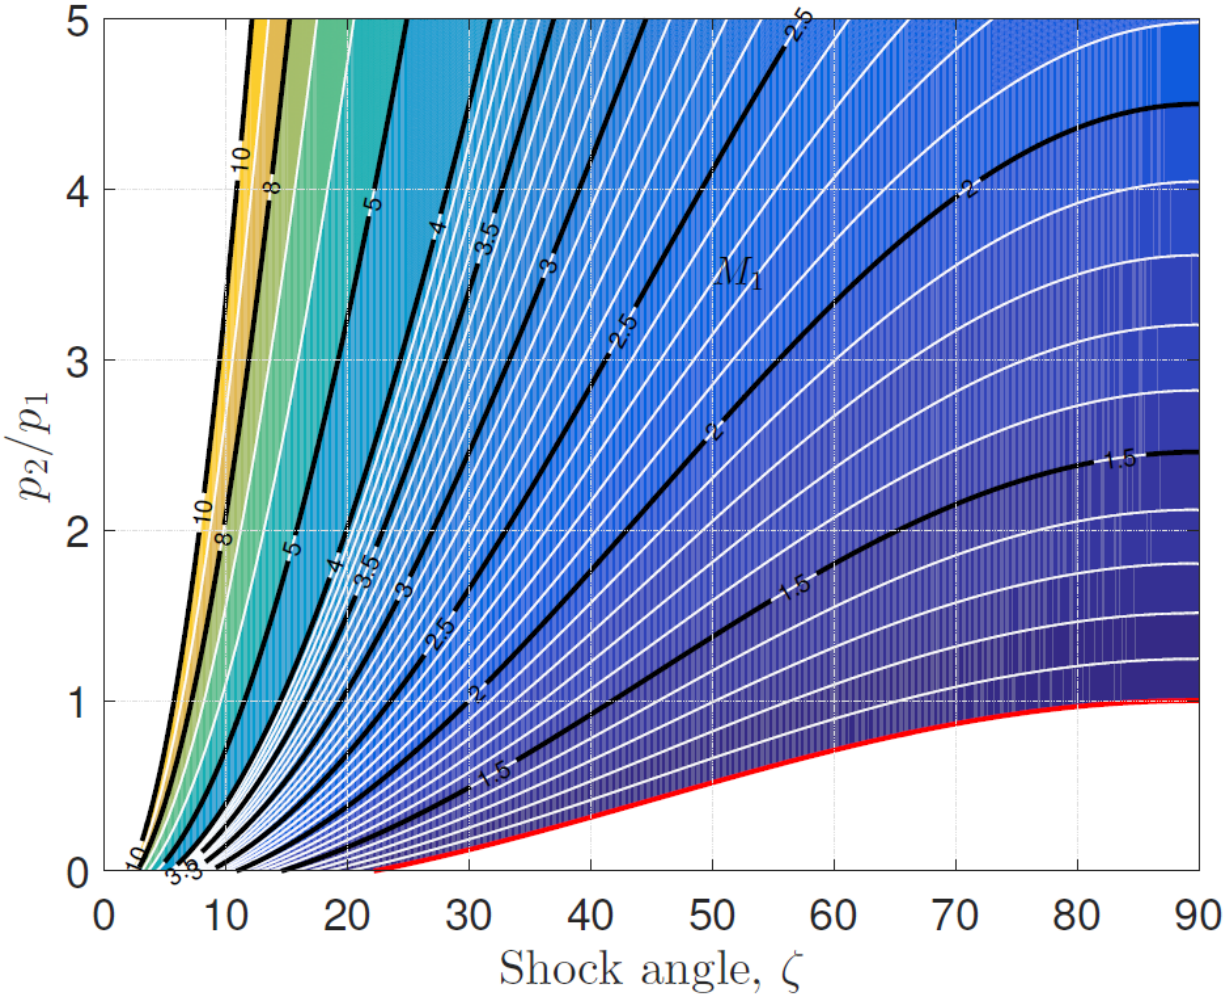
\includegraphics[width=0.9\textwidth]{./img/diagram8.png}
    \caption{Static pressure at each taps in \si{\pascal}.}
    \label{staticpressure}
\end{figure}
\begin{figure}[H]
    \centering
    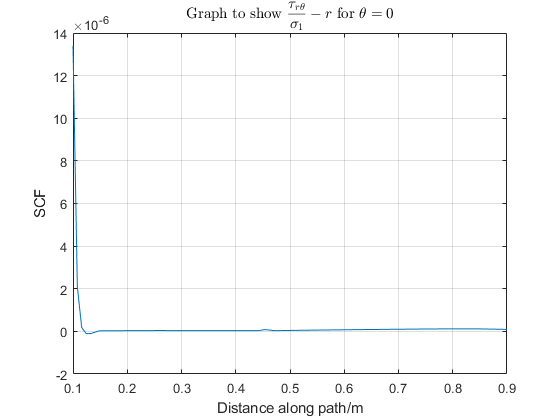
\includegraphics[width=0.9\textwidth]{./img/diagram9.png}
    \caption{Pressure coefficients at the tappings at each angle.}
\end{figure}
The pressure coefficient can be determined by the following formula:
\begin{gather}
    C_p = \frac{p - p_{\infty}}{\frac{1}{2}\rho V_{\infty}^2}\\
    p_{\infty} = -71\cdot 9.80638 = \SI{-696.253}{\pascal} \textrm{ and } V_{\infty} - \SI{20.50}{\meter\per\second}
\end{gather}
\subsection{Plot of the variation along the chord of $c_p$ at $\alpha = \SI{0}{\degree}$, \SI{4}{\degree} and \SI{14}{\degree} and discussion}
\begin{figure}[H]
    \centering
    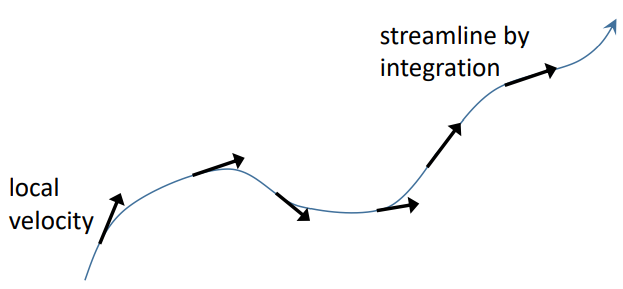
\includegraphics[width=0.85\textwidth]{./img/diagram10.jpeg}
    \caption{Upper profile variation.}
\end{figure}
\begin{figure}[H]
    \centering
    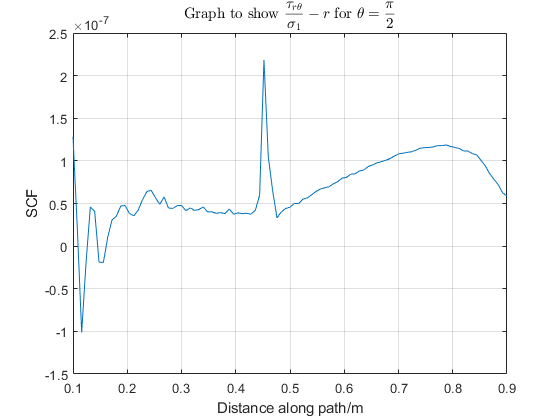
\includegraphics[width=0.85\textwidth]{./img/diagram11.jpeg}
    \caption{Lower profile variation.}
\end{figure}
We can see that for the upper profile, at angles of attack of \SI{0}{\degree} and \SI{3.6}{\degree}, the pressure coefficient along the chord are negative which represent a suction, apart from the last data point which is positive. This corresponds to the typical pressure distribution given in Fig.\ref{staticpressure}. However, for the \SI{14}{\degree} angle of attack, we can see that the last data point is negative. We can see that for the lower profile, for a \SI{3.6}{\degree} angle of attack, the pressure coefficients are always positive, which means that there is a compression region lifting the airfoil upwards. For a \SI{0}{\degree} angle of attack, the pressure coefficient is positive then turns negative before turning positive again, and is very close to 0 along the chord, meaning the compression or suction generated will be significantly smaller so the lift will be smaller. Finally, at an angle of attack of \SI{14.4}{\degree}, the pressure coefficient does not turn positive towards the end of the chord like for the two other angles, indicating the presence of a suction region. We can also see that at the angle of attack of \SI{14.4}{\degree}, the pressure coefficients at the end of the chord in the upper profile does not get closer to 0 like there would be in a typical pressure distribution. Finally we can see that until \SI{35}{\milli\meter} from the leading edge, at a \SI{3.6}{\degree} angle of attack, the pressure coefficient is approximately two times higher than at a \SI{14.4}{\degree} angle of attack.
\subsection{Determination of lift coefficient $c_L'$}
In order to find the lift coefficient, we must use the following equation:
\begin{align}
    c_L' = -\frac{1}{c} \int_0^c \left(c_p \left(\hat{n}\cdot \hat{j}\right)\right)\dif x
\end{align}
By assuming the local normal to the surface is aligned with the $y$-direction, we can simplify $\left(\hat{n}\cdot \hat{j}\right)$ based on the top and bottom surface. When looking at the top surface, we will simplify to $+1$ and the bottom to $-1$.

To integrate our pressure coefficients, we must use the trapezium rule to find an approximate for the area underneath the curve. Taking \SI{-9}{\degree}, we can integrate the top and bottom surfaces individually. The pressure coefficients at tappings 1, 2, 3 and 4 are shown below.
\begin{table}[H]
    \centering
    \label{q2bvals}
    \begin{tabular}{||c|c|c|c||}
        \hline
        \textbf{Surface tapping} & \textbf{Angle of attack} & $x/c$ & \textbf{Coefficient of pressure} \\
        \hline
        \hline
        1                        & -9                       & 0.05  & 2.1                              \\
        3                        & -9                       & 0.025 & 1.6                              \\
        2                        & -9                       & 0.01  & -2.9                             \\
        4                        & -9                       & 0.051 & -2.7                             \\
        \hline
    \end{tabular}
    \caption{Pressure coefficients at tappings 1, 2, 3 and 4.}
\end{table}
To find the area of the trapezium, we also need to know the height which is simply the difference of our two $x/c$ values at tappings 1 and 3, as well as tappings 2 and 4.
\begin{align}
    \textrm{Top area}    & = \frac{1}{2}\left(2.1 + 1.6\right)(0.025 -0.05)               \\
    \textrm{Top area}    & = 0.037                                                        \\
    \textrm{Bottom area} & = \frac{1}{2}\left(-2.9 + \left(-2.7\right)\right)(0.051-0.01) \\
    \textrm{Bottom area} & = 0.114
\end{align}
Repeating this process for all the remaining trapeziums, we can find total top and bottom areas for each angle of attack as shown below. Then, to find the lift coefficient, we simply subtract the top area from the bottom area.
\begin{table}[H]
    \centering
    \label{q2bvals2}
    \begin{tabular}{||c|c|c|c||}
        \hline
        \textbf{Angle of attack} & \textbf{Total upper area} & \textbf{Total lower area} & \textbf{Lift coefficient} \\
        \hline
        \hline
        -9                       & 0.102                     & -0.670                    & -0.773                    \\
        -7.2                     & -0.114                    & -0.523                    & -0.409                    \\
        -5.4                     & -0.279                    & -0.381                    & -0.102                    \\
        -3.6                     & -0.211                    & -0.062                    & 0.149                     \\
        -1.8                     & -0.584                    & -0.008                    & 0.577                     \\
        0                        & -0.760                    & 0.179                     & 0.939                     \\
        1.8                      & -0.979                    & 0.119                     & 1.098                     \\
        3.6                      & -1.140                    & 0.508                     & 1.648                     \\
        5.4                      & -1.335                    & 0.475                     & 1.809                     \\
        7.2                      & -1.511                    & 0.692                     & 2.203                     \\
        9                        & -1.663                    & 0.824                     & 2.488                     \\
        10.8                     & -1.783                    & 0.925                     & 2.707                     \\
        12.6                     & -1.829                    & 0.985                     & 2.814                     \\
        14.4                     & -2.091                    & 0.358                     & 2.449                     \\
        16.2                     & -2.118                    & 0.361                     & 2.479                     \\
        18                       & -2.076                    & 0.331                     & 2.406                     \\
        \hline
    \end{tabular}
    \caption{Lift coefficients.}
\end{table}
\subsection{Plot of the lift coefficient, $c_L'$ against $\alpha$ and comparison to NACA}
Based on the graph from the NACA Technical Notes 2074 (Fig.\ref{nacagraph}), our values for the lift coefficient can be compared.
\begin{figure}[H]
    \centering
    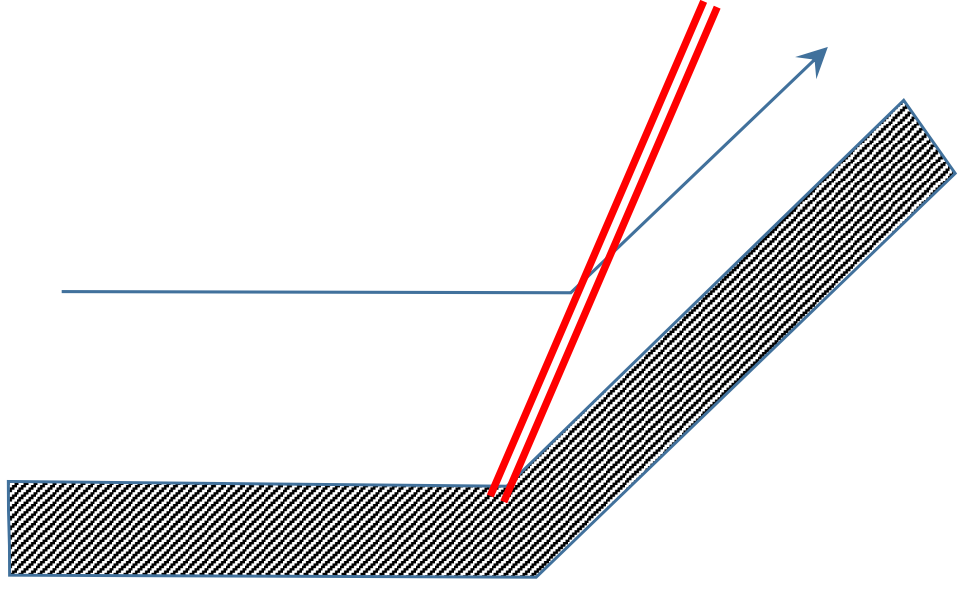
\includegraphics[width = 0.9\textwidth]{./img/diagram20.png}
    \caption{Lift coefficient from NACA Technical Notes 2074.}
    \label{nacagraph}
\end{figure}
Plotting both sets of results on a single graph, we arrive at Fig.\ref{liftcoeffgraphs}
\begin{figure}[H]
    \centering
    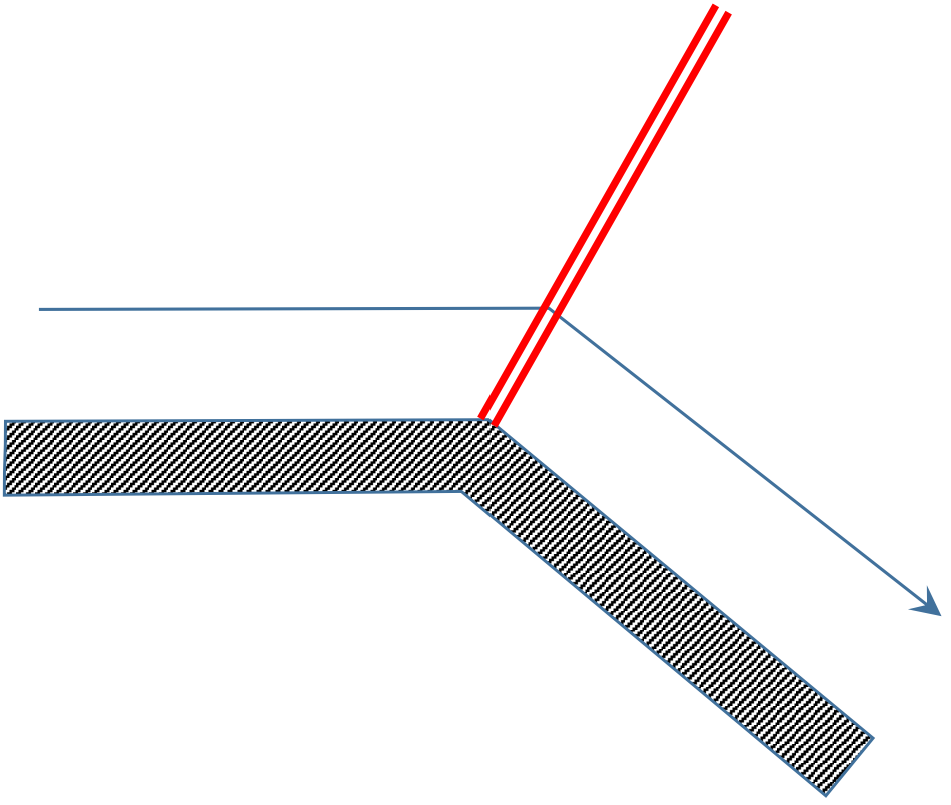
\includegraphics[width = 0.6\textwidth]{./img/diagram21.png}
    \caption{Experimental and NACA lift coefficients.}
    \label{liftcoeffgraphs}
\end{figure}
\subsection{Discussion on what an aerofoil stall is}
Both sets of results follow a similar trend where the lift coefficient rises uniformly. Then at a critical angle of around \SI{15}{\degree}, it suddenly drops. This phenomenon is known as stalling and is a result of the angle of attack being too large. Beyond the critical angle, flow over the top surface of an aerofoil becomes turbulent thus increasing drag and reducing lift as shown in Fig.\ref{liftcoeffgraphs}.
\section{Part 2 - Conformal Mapping}
\subsection{Shape change of the cylinder when the parameters, $x_c$, $y_c$ and $\lambda$ are varied}
Varying the value of $\lambda$ between 0 and 1 compressed the cylinder into an elliptical shape and approached the shape of a line with length $4r$ at $\lambda = 1$. For values greater than 1, the shape produced was an ellipse and an increase in $\lambda$ provided a scaling effect. Changing $x_c$ would change the shape of the cylinder from elliptical to a symmetrical tear drop shape (aerofoil shape), with one edge becoming more pinched and the other more rounded. Changing $x_c$ when $\lambda < 1$ would pinch the right side, whereas for $\lambda >1$ it would pinch the left side. Changing $y_c$ would skew the aerofoil into a curved shape, becoming unsymmetrical. This would result in one of the profiles of the wing becoming concave.
\subsection{Determination of the values of $x_c$ and $y_c$ }
Using the following equation, we can derive $\lambda$ as a function of $x_c$:
\begin{align}
    \lambda = \left(R - \sqrt{x_c^2 + y_c^2}\right) \\
\end{align}
$y_c = 0$ because our NACA-0012 aerofoil is uncambered. $R = 1$. Therefore:
\begin{align}
    \lambda   & = \left(1-\sqrt{x_c^2}\right) \\
    \lambda   & = \left(1-x_c\right)          \\
    \lambda^2 & = \left(1-x_c\right)^2
\end{align}
After iteratively changing the value of $x_c$, we found that a value of $x_c = -0.94$ and $\lambda^2 = 0.820836$ produced an aerofoil closely matching the NACA-0012. This is shown in Fig.\ref{mappedaerofoil}.
\begin{figure}[H]
    \centering
    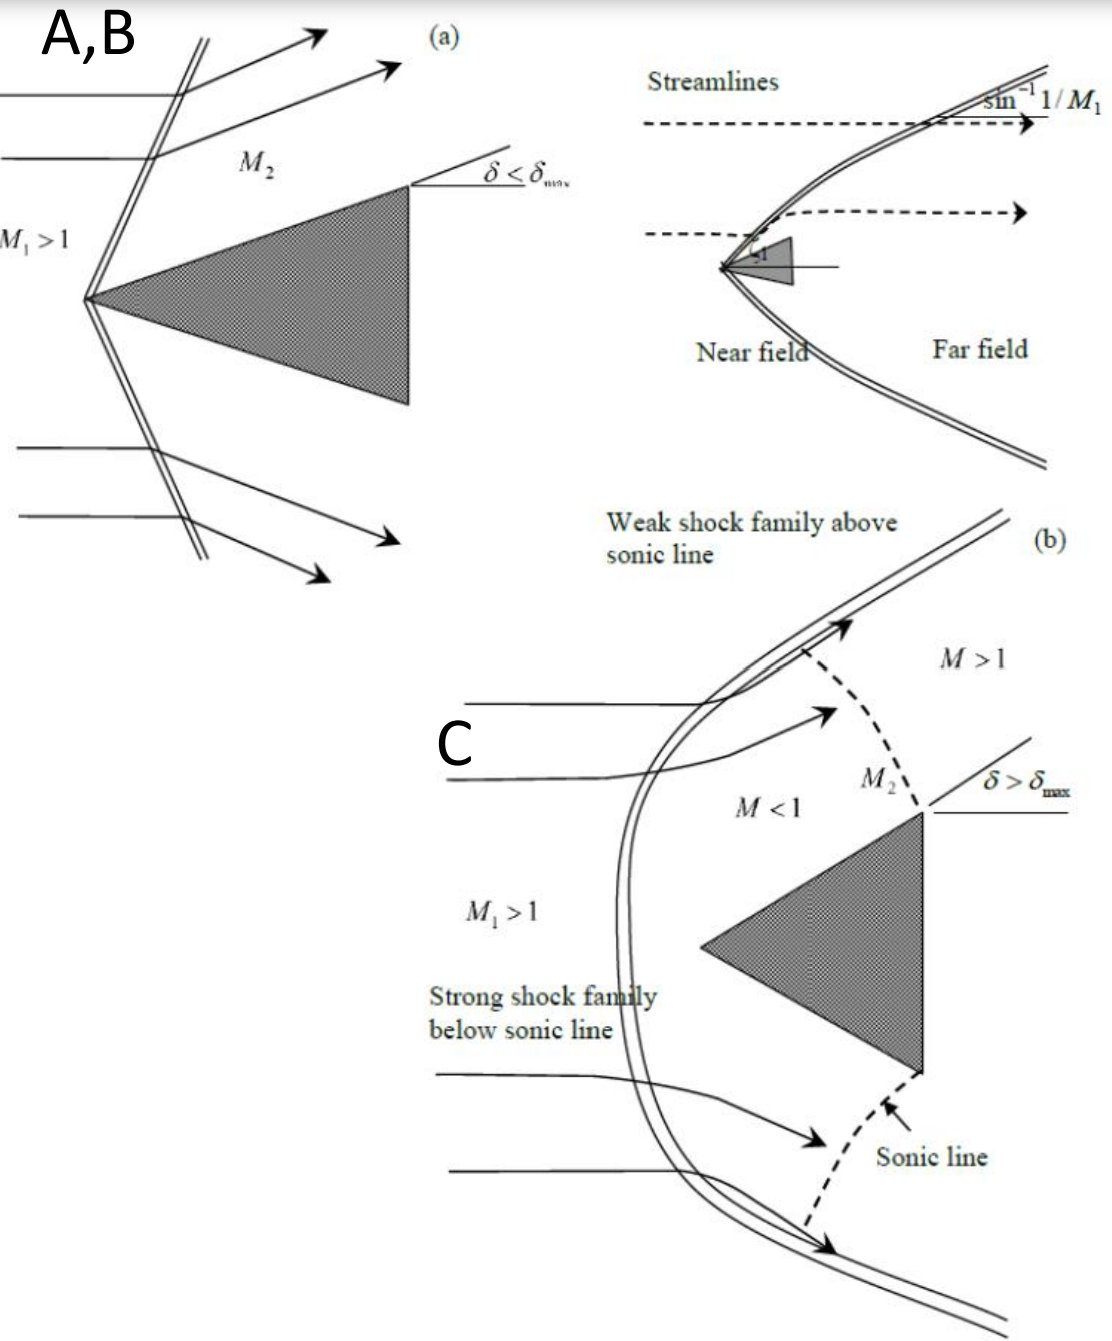
\includegraphics[width = 0.6\textwidth]{./img/diagram15.png}
    \caption{Aerofoil with parameters $x_c = -0.94$ and $\lambda^2 = 0.820836$.}
    \label{mappedaerofoil}
\end{figure}
To calculate the chord length, the minimum and maximum values were taken from the NACA profile scaled and shifted, x column in the excel sheet. This yielded -1.85 and 1.85. Hence, our chord length, $c$, is \SI{3.7}{\metre}. A similar approach was taken to find $t_{max}$. The excel sheet yielded -0.222 and 0.222 as our minimum and maximum $y$ values. Hence, $t_{max} = \SI{0.444}{\metre}$.
\subsection{Plot of the streamlines around the cylinder in the (x, y) plane for $\alpha = 0$ and $\psi = \pm 0.1$}
The stream function of the flow around a cylinder of radius, $R$ is given by Eq.\ref{streamfunction}:
\begin{align}
    \psi = U_{\infty}r\sin\left(\theta\right) \left(1 - \frac{R^2}{r^2}\right) + \frac{\Gamma}{2\pi}\log\left(r\right)\label{streamfunction}
\end{align}
where a cylindrical coordinate system $(r,\theta)$ is used.
The lift of the cylinder is proportional to the circulation, $\Gamma$, as shown in Eq.\ref{liftcirc}:
\begin{align}
    L = \rho U_{\infty} \Gamma \label{liftcirc}
\end{align}
Substituting $\psi = \pm 0.1$, $\alpha = 0$, $U_{\infty} = 1$ and $R=1$ into Eq.\ref{streamfunction}:
\begin{align}
    \pm 0.1 = r\sin\left(\theta\right) \left(1-\frac{1}{r^2}\right) + \frac{\Gamma}{2\pi} \log\left(r\right) \label{streamfunction2}
\end{align}
From our cylindrical coordinate system, we know that $x=r\cos\theta$ and $y = r\sin\theta$. Hence, we can derive that $x^2 + y^2 = r^2$. We can also rearrange Eq.\ref{liftcirc} in terms of $\Gamma$. Substituting these values into Eq.\ref{streamfunction2}:
\begin{align}
    \pm 0.1 = y\left(1-\frac{1}{x^2 + y^2}\right)\label{streamfunction3}
\end{align}
We can derive three equations now, shown below:
\begin{align}
    0.1  & = y\left(1-\frac{1}{x^2 + y^2}\right) \\
    -0.1 & = y\left(1-\frac{1}{x^2 + y^2}\right) \\
    1    & = x^2 + y^2
\end{align}
These were plotted in MATLAB with the following code:
\lstset{language=Matlab,%
    %basicstyle=\color{red},
    breaklines=true,%
    morekeywords={matlab2tikz},
    keywordstyle=\color{blue},%
    morekeywords=[2]{1}, keywordstyle=[2]{\color{black}},
    identifierstyle=\color{black},%
    stringstyle=\color{mylilas},
    commentstyle=\color{mygreen},%
    showstringspaces=false,%without this there will be a symbol in the places where there is a space
    numbers=left,%
    numberstyle={\tiny \color{black}},% size of the numbers
    numbersep=9pt, % this defines how far the numbers are from the text
    emph=[1]{for,end,break},emphstyle=[1]\color{red}, %some words to emphasise
    %emph=[2]{word1,word2}, emphstyle=[2]{style},    
}
\lstinputlisting{m/MECH0011FMLQ2c.m}
This produced the following plot:
\begin{figure}[H]
    \centering
    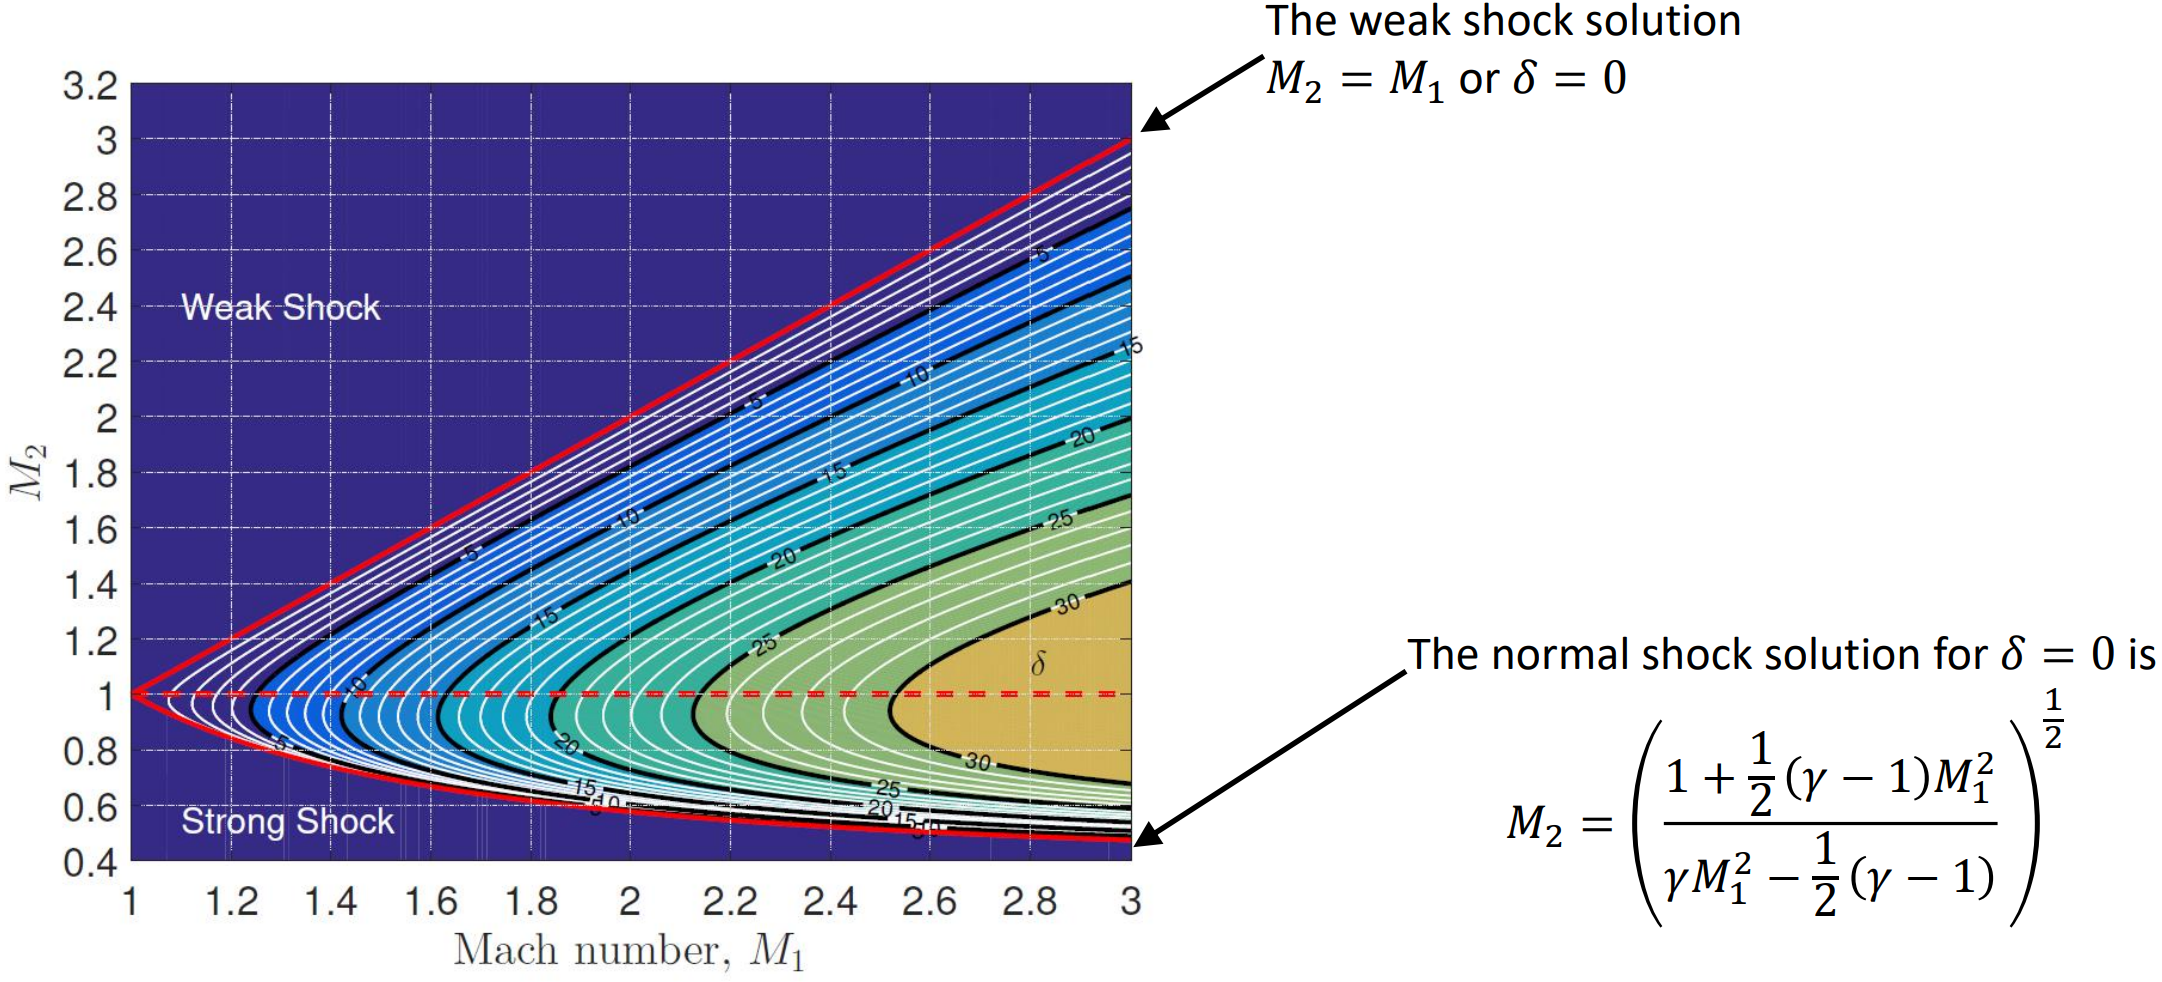
\includegraphics[width = 0.6\textwidth]{./img/diagram16.png}
    \caption{Plot of streamlines around cylinder.}
\end{figure}
\subsection{Use of Joukowsky transformation to obtain the streamlines around the aerofoil in the $\left(\xi, \zeta \right)$ plane.}
We know:
\begin{align}
    G(z)    & = z + \frac{\lambda^2}{z}  \\
    \lambda & = R - \sqrt{x_c^2 + y_c^2} \\
    z = \left(x-x_c\right) + i\left(y-y_c\right)
\end{align}
We also know that $y_c = 0$:
\begin{align}
    \lambda & = R - \left| x_c \right|  \\
    z       & = \left(x-x_c\right) + iy
\end{align}
$x$ and $y$ in cylindrical coordinates:
\begin{align}
    x & = R\cos\theta \\
    y & = R\sin\theta
\end{align}
Joukowsky transform, $G(z) = w$:
\begin{align}
    w = R\cos\theta - x_c + iR\sin\theta + \frac{\left(R-\left|x_c\right|\right)^2}{R\cos\theta - x_c + iR\sin\theta}
\end{align}
Inputting $R=1$:
\begin{align}
    w & = \cos\theta - x_c + i\sin\theta + \frac{\left(1-\left|x_c\right|\right)^2}{\cos\theta - x_c + i\sin\theta}                                                                             \\
    w & = \cos\theta - x_c + i\sin\theta + \frac{\left(1-\left|x_c\right|\right)^2}{\cos\theta - x_c + i\sin\theta} \cdot \frac{\cos\theta - x_c - i\sin\theta}{\cos\theta - x_c - i\sin\theta} \\
    w & = \cos\theta - x_c + i\sin\theta + \frac{\left(1-\left|x_c\right|\right)^2 \cdot \left(\cos\theta - x_c - i\sin\theta\right)}{\cos^2\theta -2x_c\cos\theta + x_c^2 + \sin^2\theta}      \\
    w & = \cos\theta - x_c + i\sin\theta + \frac{\left(1-\left|x_c\right|\right)^2 \cdot \left(\cos\theta - x_c - i\sin\theta\right)}{1 -2x_c\cos\theta + x_c^2}                                \\
\end{align}
Separating into real and imaginary components:
\begin{align}
    w = \left(\cos\theta - x_c + \frac{\left(1-\left|x_c\right|\right)^2 \cdot \left(\cos\theta - x_c\right)}{1 -2x_c\cos\theta + x_c^2}\right) + i\left(\sin\theta + \frac{-\left(1-\left|x_c\right|\right)^2 \cdot \sin\theta}{1 -2x_c\cos\theta + x_c^2}\right)
\end{align}
We know that $w = \xi + i\zeta$:
\begin{align}
    \xi   & = \left(\cos\theta - x_c + \frac{\left(1-\left|x_c\right|\right)^2 \cdot \left(\cos\theta - x_c\right)}{1 -2x_c\cos\theta + x_c^2}\right) \\
    \zeta & = \left(\sin\theta + \frac{-\left(1-\left|x_c\right|\right)^2 \cdot \sin\theta}{1 -2x_c\cos\theta + x_c^2}\right)
\end{align}
Joukowsky transform plotted in MATLAB with the following code:
\lstset{language=Matlab,%
    %basicstyle=\color{red},
    breaklines=true,%
    morekeywords={matlab2tikz},
    keywordstyle=\color{blue},%
    morekeywords=[2]{1}, keywordstyle=[2]{\color{black}},
    identifierstyle=\color{black},%
    stringstyle=\color{mylilas},
    commentstyle=\color{mygreen},%
    showstringspaces=false,%without this there will be a symbol in the places where there is a space
    numbers=left,%
    numberstyle={\tiny \color{black}},% size of the numbers
    numbersep=9pt, % this defines how far the numbers are from the text
    emph=[1]{for,end,break},emphstyle=[1]\color{red}, %some words to emphasise
    %emph=[2]{word1,word2}, emphstyle=[2]{style},    
}
\lstinputlisting{m/MECH0011FMLQ2d.m}
This produced the following plot:
\begin{figure}[H]
    \centering
    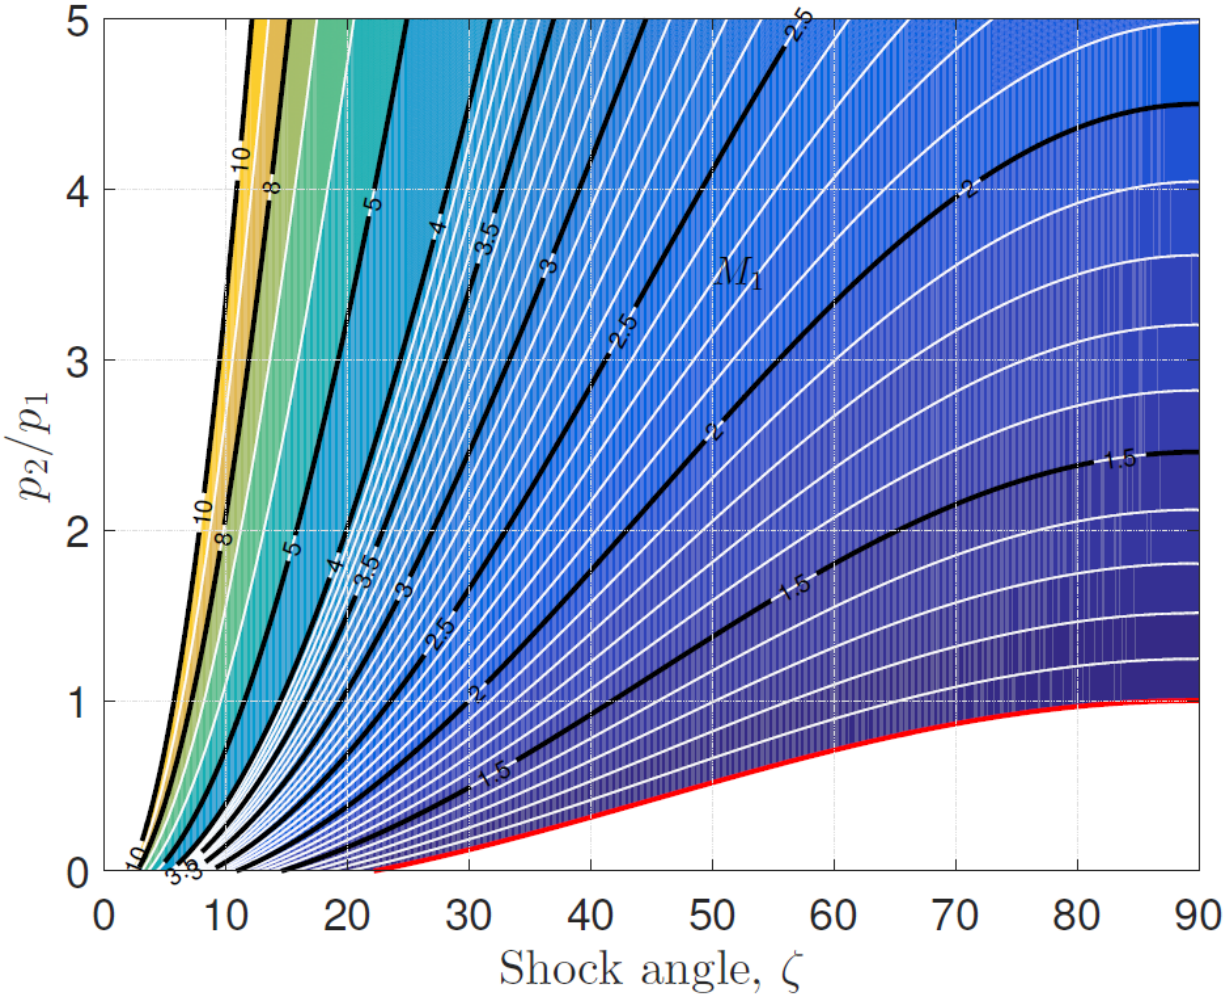
\includegraphics[width = \textwidth]{./img/diagram17.png}
    \caption{Plot of Joukowsky transformed streamlines.}
\end{figure}
\subsection{Determination of the circulation $\Gamma$ as a function of the angle of incidence $\alpha$ for a cylinder using Kutta condition. Discussion on the condition that the Kutta condition imposes}
We impose the Kutta condition when we have unrealistic streamlines e.g. Fig.\ref{unrealisticstreamline}
\begin{figure}[H]
    \centering
    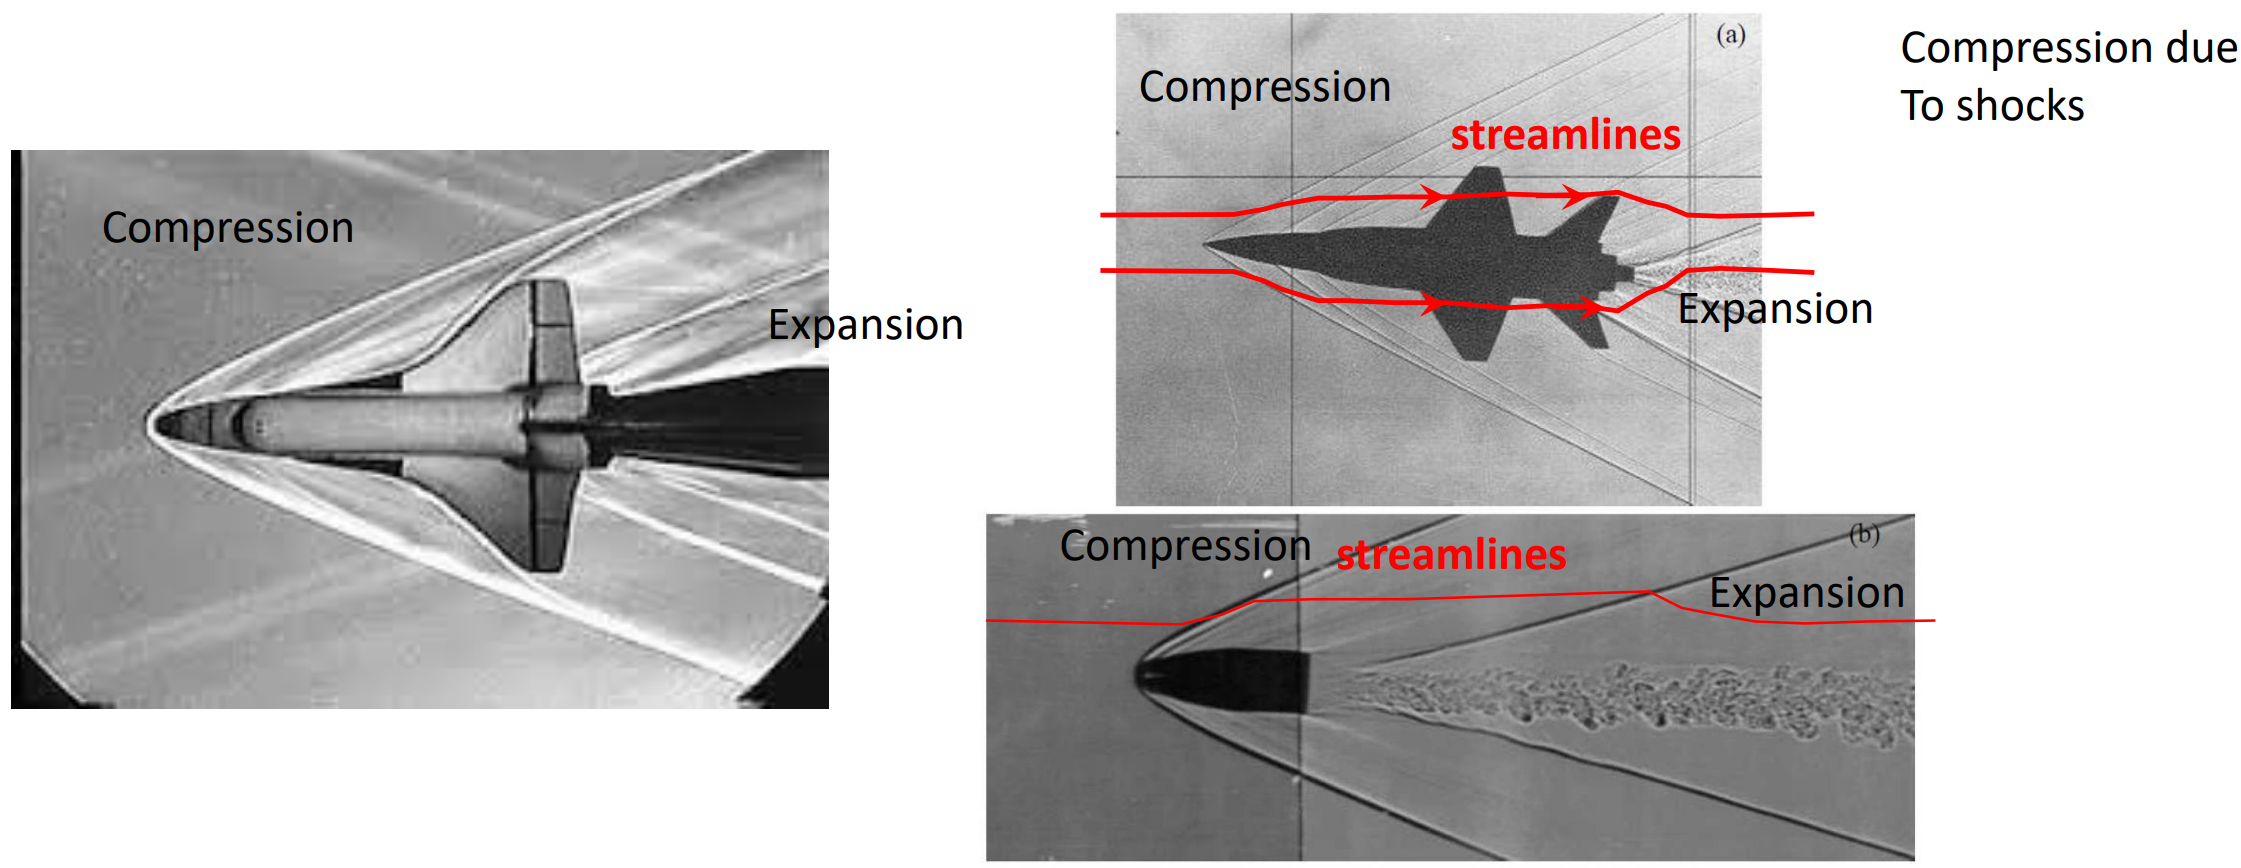
\includegraphics[width = 0.8\textwidth]{./img/diagram18.png}
    \caption{Unrealistic streamlines.}
    \label{unrealisticstreamline}
\end{figure}
This streamline is unrealistic because to curl around the trailing edge cusp, the speed goes to infinity. This is impossible and flow separation would occur instead. For a given angle of coincidence, the circulation has to be selected by imposing that the back stagnation point and the aerofoil trailing edge coincide, as shown in Fig.\ref{goodkutta}
\begin{figure}[H]
    \centering
    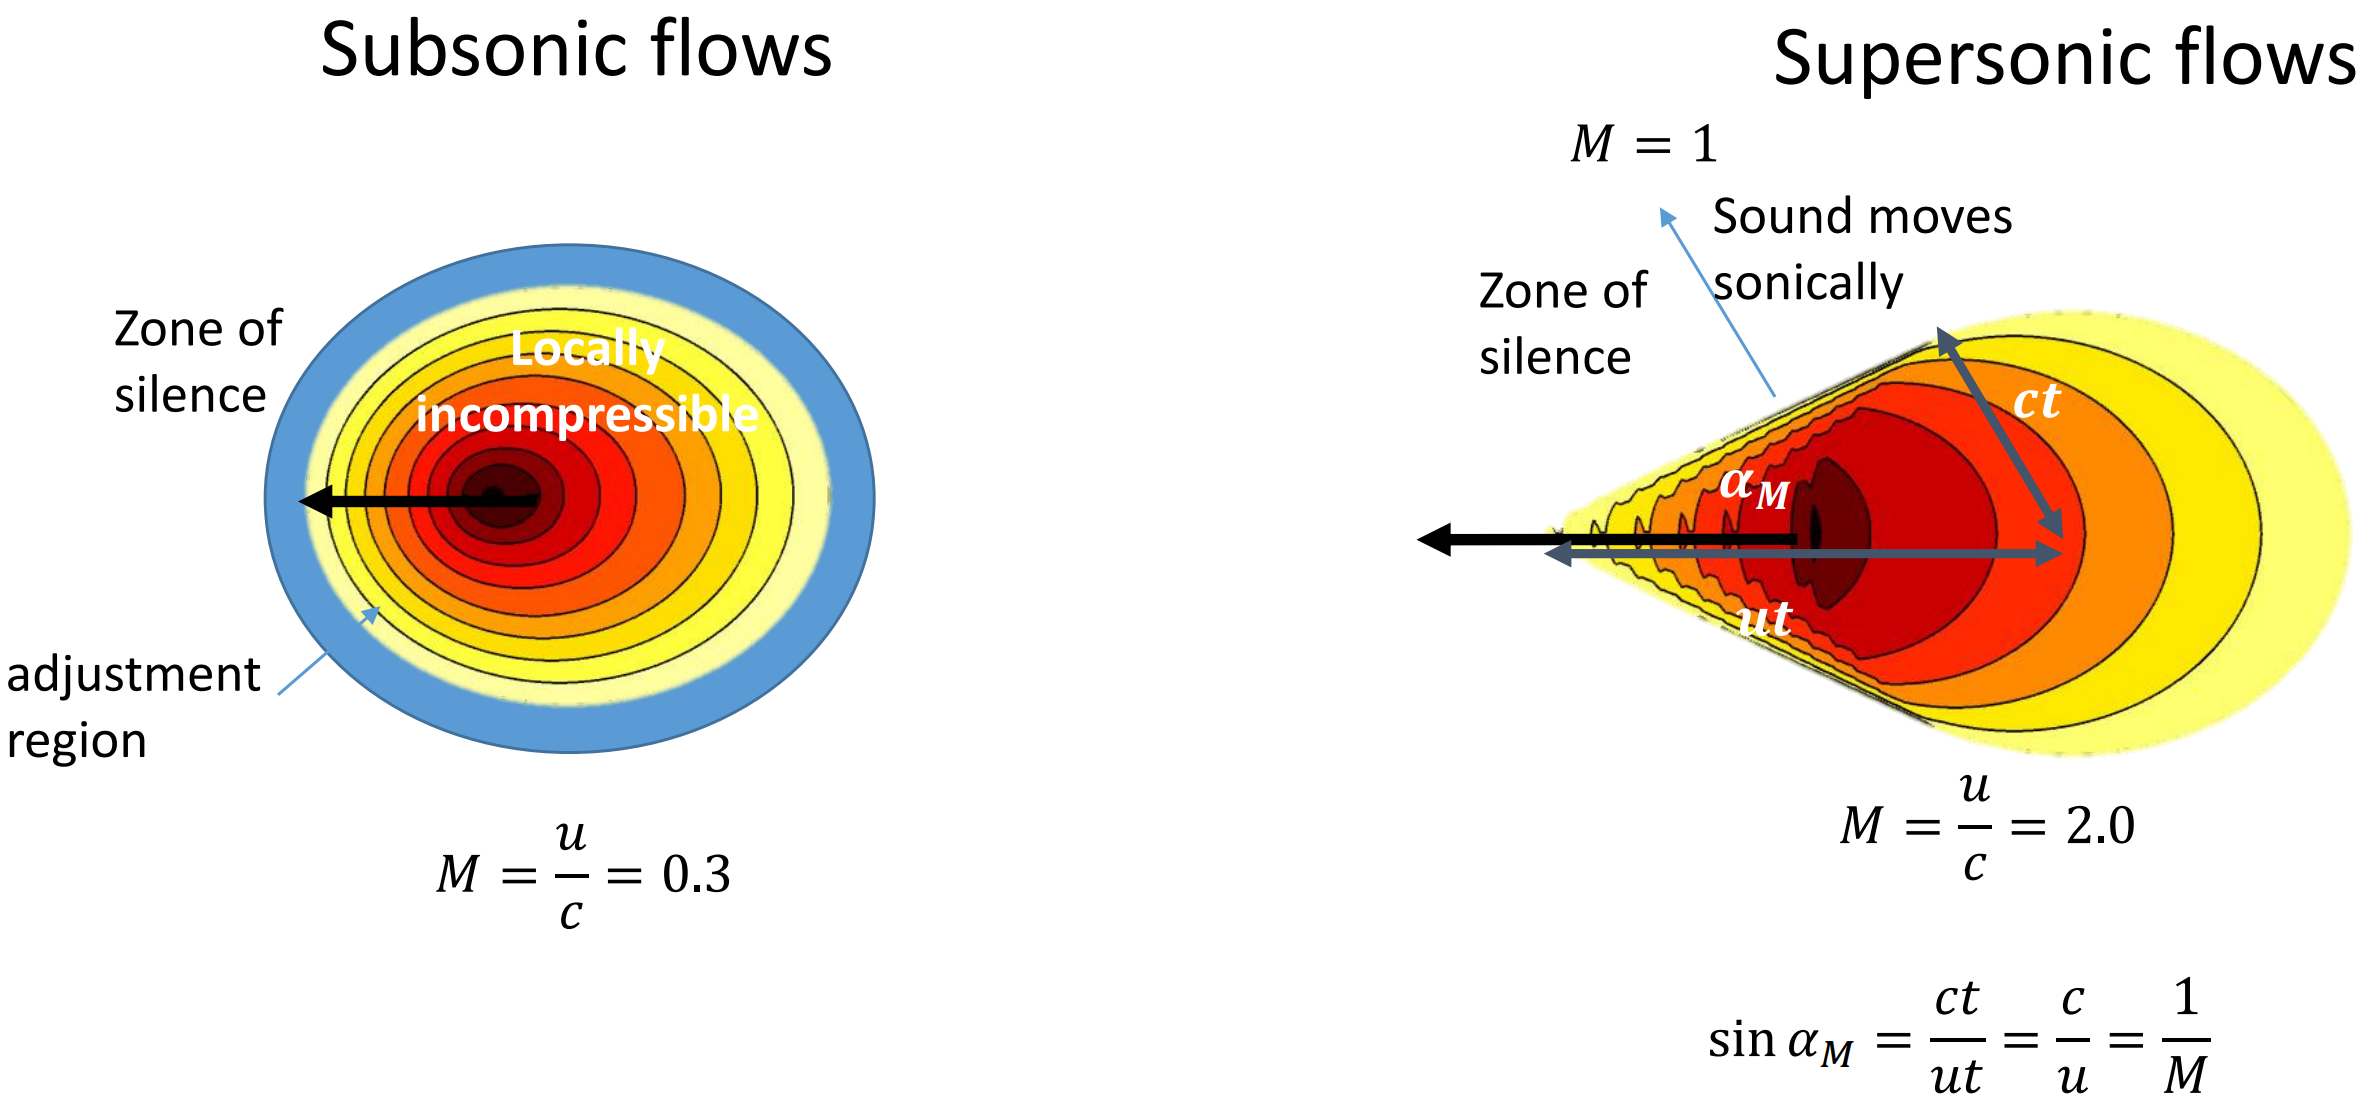
\includegraphics[width = 0.8\textwidth]{./img/diagram19.png}
    \caption{Back stagnation point coinciding with trailing edge of aerofoil.}
    \label{goodkutta}
\end{figure}
Some requirements for the Kutta condition are:
\begin{itemize}
    \item Inviscid flow in the region surrounding the aerofoil
    \item Back stagnation point and aerofoil trailing edge coincide
    \item Valid for $\alpha < \alpha_{crit}$ where $\alpha_{crit}$ is the critical angle of attack where stalling occurs.
    \item Fluid flowing on the top and bottom of the aerofoil meets smoothly at the trailing edge.
\end{itemize}
Determining $\Gamma$ as a function of $\alpha$. Streamline function:
\begin{align}
    \psi = U_{\infty}r \sin\left(\theta-\alpha\right) \left(1 - \frac{R^2}{r^2}\right) + \frac{\Gamma}{2\pi}\log r
\end{align}
Velocity components:
\begin{align}
    u_{\theta} & = -\frac{\partial \psi}{\partial r}                                                                   \\
    u_{\theta} & = -U_{\infty} \sin\left(\theta-\alpha\right) \left(1 + \frac{R^2}{r^2}\right) - \frac{\Gamma}{2\pi r} \\
    u_r        & = \frac{1}{r} \frac{\partial \psi}{\partial \theta}                                                   \\
    u_r        & = U_{\infty} r\cos\left(\theta-\alpha\right) \left(1-\frac{R^2}{r^2}\right)
\end{align}
On the cylinder $r=R$:
\begin{align}
    u_{\theta} & = -2U_{\infty} \sin\left(-\alpha\right) - \frac{\Gamma}{2\pi R} \\
    u_r        & = 0
\end{align}
Kutta condition:
\begin{align}
    u_{\theta} \left(\theta = 0\right)                   & = 0                           \\
    \Gamma = -4\pi U_{\infty} R \sin\left(-\alpha\right) & = 4\pi U_{\infty} R\sin\alpha
\end{align}
$R=1$ and $U_{\infty} =1$:
\begin{align}
    \Gamma = 4\pi \sin\alpha
\end{align}
\subsection{Determination of the lift, $L$, and a plot of the lift coefficient, $c_L'$, of the aerofoil as a function of the angle of incidence}
\begin{align}
    \Gamma & = 4\pi R U_{\infty} \sin a                                                                                                                    \\
    L      & = \rho U_{\infty} \Gamma = 4\pi R \rho U_{\infty}^2 \sin a                                                                                    \\
    c_L'   & = \frac{L}{\frac{1}{2}\rho U_{\infty}^2 c} = \frac{4\pi R \rho U_{\infty}^2 \sin a}{\frac{1}{2}\rho U_{\infty}^2 c} = \frac{4\pi R \sin a}{c}
\end{align}
$R=1$ and $c=3.6$. Hence:
\begin{align}
    c_L' = \frac{4\pi}{3.6}\sin a \label{liftcoeff}
\end{align}
\begin{figure}[H]
    \centering
    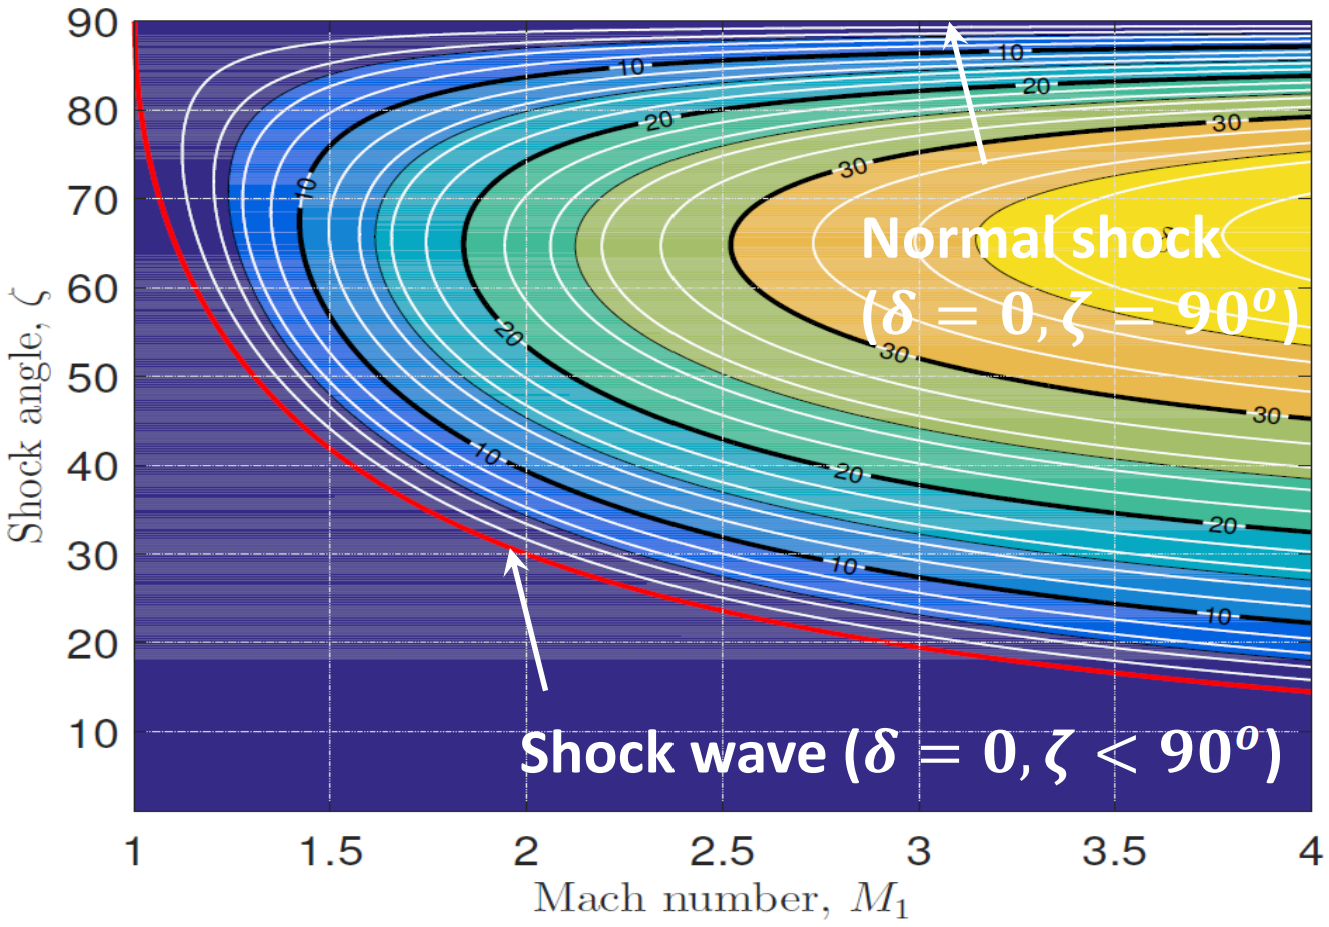
\includegraphics[width=0.5\textwidth]{./img/diagram12.png}
    \caption{Plot of Eq.\ref{liftcoeff}.}
    \label{liftcoeffplot}
\end{figure}
The plot in Fig.\ref{liftcoeffplot} is, as expected, a straight line. We know from Eq.\ref{liftcoeff} that it is a sine function with a scalar factor. We also know from the small angle approximation that $\sin a \approx a$ for small $a$, leading to our lift coefficient being: $c_L' = \frac{8\pi}{3.6}a$, which is a straight line with a fixed gradient.
\subsection{Compare the plot of the lift coefficient, $c_L'$, with that obtained from experimental analysis. Discuss on the validity of conformal mapping over the range of angles investigated}
\begin{figure}[H]
    \centering
    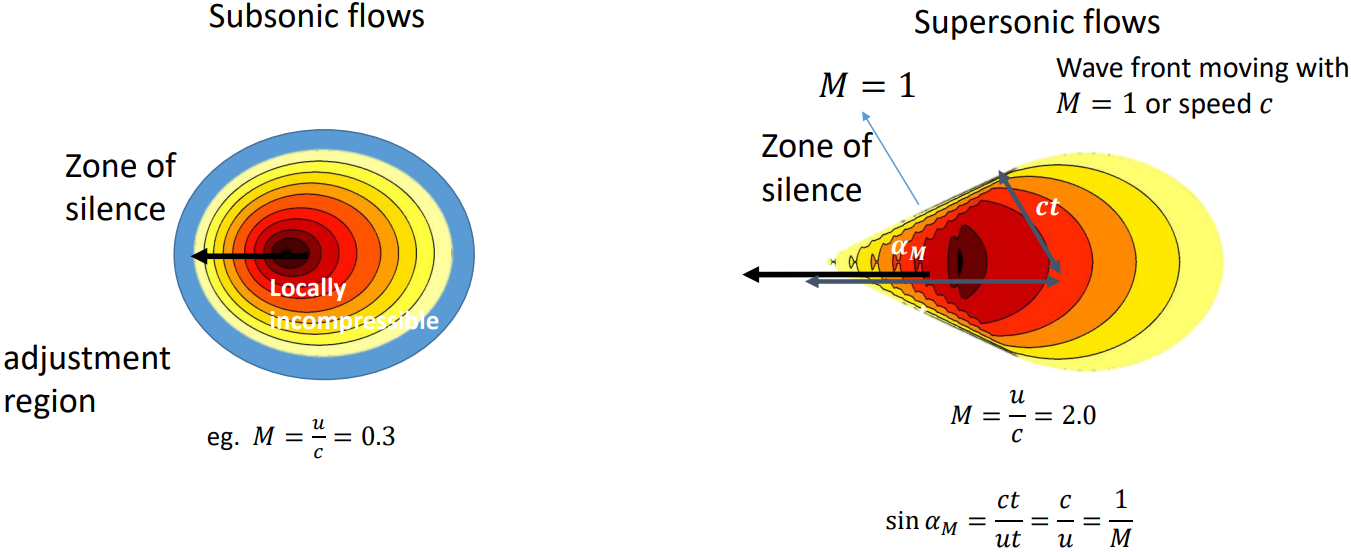
\includegraphics[width=0.6\textwidth]{./img/diagram13.png}
    \caption{Plot of calculated $c_L$ (blue) and of experimental $c_L$ (red).}
\end{figure}
\begin{figure}[H]
    \centering
    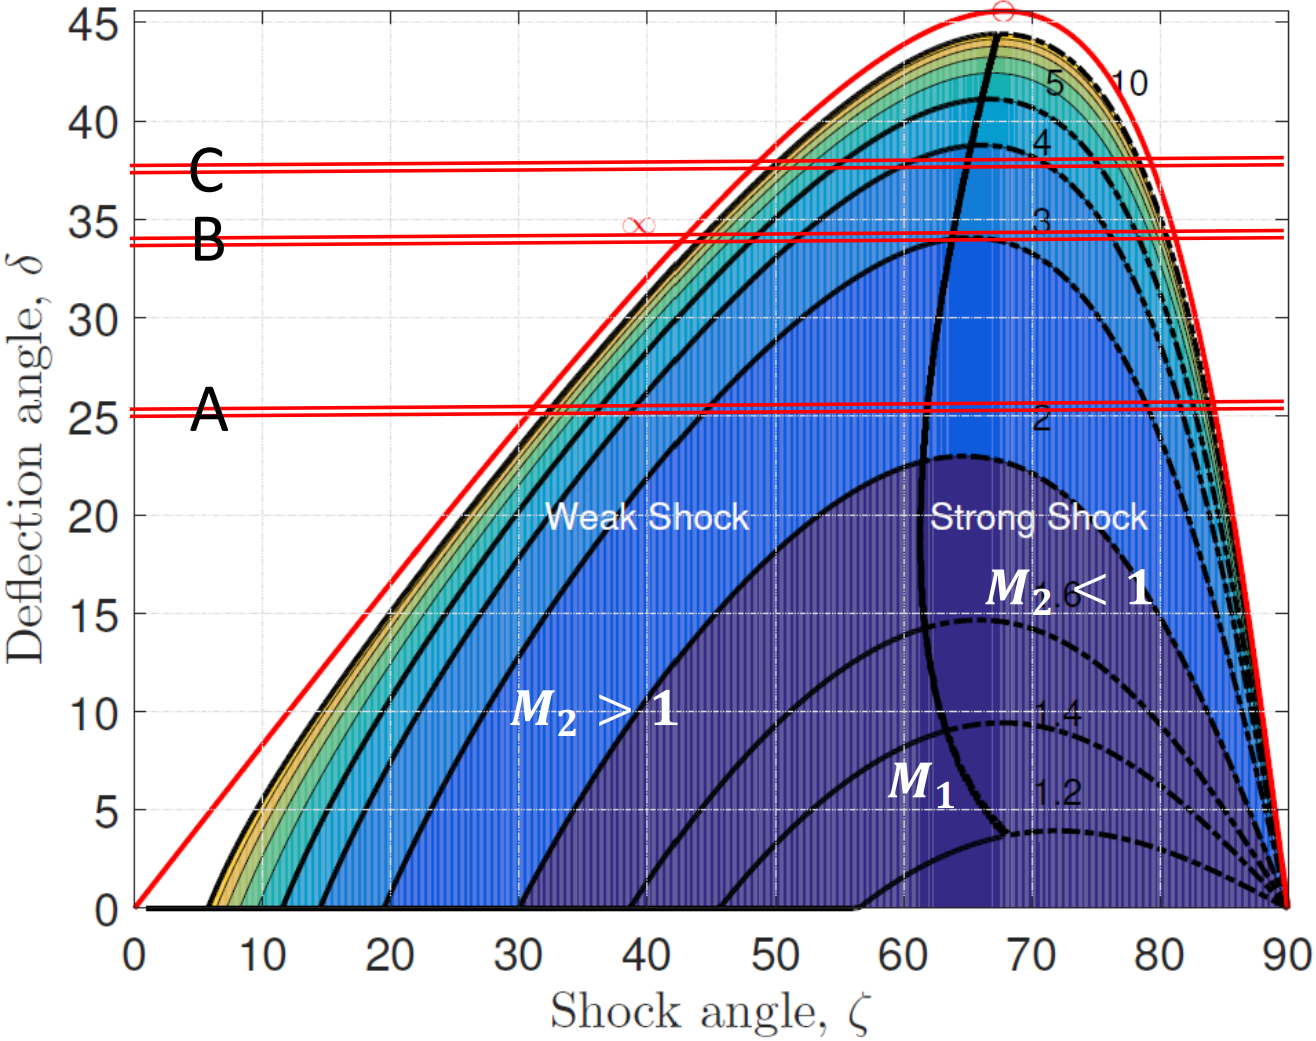
\includegraphics[width=0.6\textwidth]{./img/diagram14.png}
    \caption{Manometer values for $a=\SI{16.2}{\degree}$ (left) and $a = \SI{18}{\degree}$ (right).}
\end{figure}
In general, conformal mapping is accurate to use. The two lines do not completely overlap, but the two lines are very close to each other before being intercepted, as no flow separation occurs. After the intercept point, the experimental $c_L$ is still on the track of the theoretical $c_L$, but when the incident angle is between \SI{16.2}{\degree} and \SI{18}{\degree}, the experimental $c_L$ suddenly drops. This is because when $a=\SI{16.2}{\degree}-\SI{18}{\degree}$, a stall occurs and flow separation occurs. When $a$ is greater than the critical angle of attack, boundary layer separation will occur on the upper surface of the wing. This is due to the existence of an unfavourable pressure gradient and wall stress equals zero at the flow separation point. As a result, the suction pressure is lost and the pressure difference will decrease and the lift will drop. From the experimental data, it can be observed that the pressure difference decreases. When $a$ is between \SI{16.2}{\degree} and \SI{18}{\degree}, the pressure difference drops suddenly, which means that flow separation has occurred.